\chapter{Introduction}\label{cha:introduction}

This section introduces the project, provides context for why it was undertaken, and presents some important background information. The necessity of crack propagation analysis within the civil aerospace sector is discussed first, followed by an explanation of the potential benefits that the project could deliver within this area. The aims \& objectives of the project are then presented, followed by a summary of the methodology used, along with a methodology diagram. The final section of the chapter provides an overview of the structure of the remainder of the thesis.

\newpage
\section{Background}\label{sec:background}

Modern civil aircraft must meet multiple -- sometimes conflicting -- requirements: they must be as light as possible in order to maximise fuel efficiency, durable enough to achieve the long service life expected by customers, and compliant with the stringent safety standards demanded by the aviation authorities. In order to design aircraft that meet these requirements, it is necessary to be able to accurately predict the fatigue lives of structural components. This requires understanding of where cracks are likely to initiate, and how quickly they will grow. Accurate fatigue life predictions provide assurance that an aircraft will be able to achieve its specified service life while maintaining an extremely low risk of fatigue failure, and minimising the amount of unnecessary mass added to the aircraft's structure. The study and analysis of crack initiation and growth within airframe structures falls within the engineering discipline of fatigue and damage tolerance analysis. Fatigue and damage tolerance analysis incorporates many distinct processes --  including physical testing,  manufacturing inspections, and analysis of in-service data -- as shown in Figure \ref{fig:f_and_dt_summary}. However, the focus of this thesis is on the process of crack propagation life calculation This process aims to predict the rate of fatigue crack growth within a structure, in order to ensure that it is inspected and retired in a timely manner.

\begin{figure}[H]
	\centering
	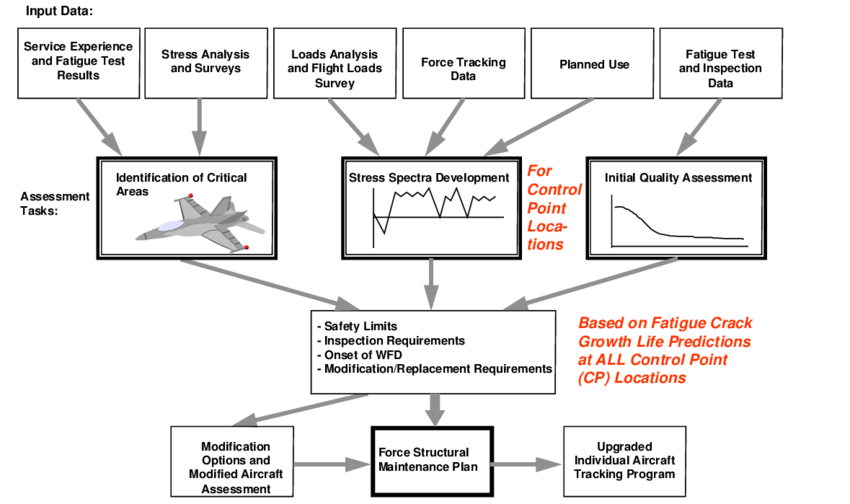
\includegraphics[width=\textwidth]{f_and_dt_summary.png}
	\caption{An overview of the end-to-end fatigue and damage tolerance analysis process. This thesis focuses solely on the topic of crack propagation analysis. \cite{gallagher_damage_2005}}
	\label{fig:f_and_dt_summary}
\end{figure}

A variety of methods are available for performing crack propagation analysis, ranging from simple and conservative methods used in general applications, to highly complex methods used in specialised applications, where a high degree of accuracy is required or where the available margin for error is limited. Many aircraft primary structures -- such as the wing skins, stringers, and spars -- are thin-walled, and can therefore be approximated as two-dimensional structures under plane-stress conditions. Two-dimensional structures are relatively simple to analyse, because analytical and empirical methods are available which can be used to obtain reasonable and conservative approximations of crack propagation rates. However, some critical primary structures are too thick to be approximated as two-dimensional -- these include the reinforcing elements around the main landing gear, for example, which are some of the most highly loaded areas on the entire aircraft. For these areas, more complex approaches are necessary, which normally involve the use of numerical methods -- particularly finite element analysis.

Although finite element analysis provides a highly effective method of calculating crack propagation rates, it generally introduces significant complexity when compared to the standard empirical and analytical methods. An engineer with a specialised skill-set is required, and significantly more time is necessary to validate that the finite element model accurately represents the real-world structure. One of the key drivers of this additional complexity is the geometry creation and meshing process. When using simpler analytical methods, a global finite element model (GFEM) may be used. A GFEM is a finite element model which models an entire section of an aircraft's structure -- such as a wing, fuselage section, or empennage -- in coarse detail, using large shell and bar elements on the order of 100 mm \cite{dharmasaroja_load_2017}. Rather than providing specific loads at each feature, a GFEM provides average loads in the general vicinity of the feature. These loads are used as inputs for idealised analytical methods, using solutions obtained from reference books or software such as NASGRO. These solutions use the remote loading along with idealised two-dimensional geometry to calculate the stress intensity factor for the feature, and therefore predict the crack propagation rate. Since a GFEM only provides average loads, it is unsuitable for performing crack propagation analysis calculations directly. For this to be accomplished, a finer DFEM (detailed finite element model) needs to be created for the specific feature being analysed, with mesh elements on the order of 1 mm or less. The difference in idealisation between a GFEM and a DFEM is presented in Figure \ref{fig:gfem_dfem}.

\begin{figure}[H]
	\centering
	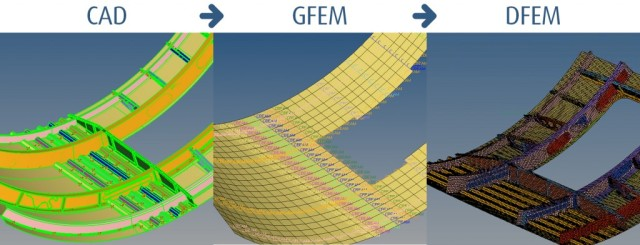
\includegraphics[width=\textwidth]{gfem_dfem.png}
	\caption{An overview of the difference in structure idealisation between a GFEM and a DFEM. The CAD model captures the geometry accurately. The GFEM idealises the CAD model using a coarse mesh of shell and bar elements, while the DFEM uses a fine mesh of solid elements \cite{wasserman_altair_2016}.}
	\label{fig:gfem_dfem}
\end{figure}

\newpage
Creating a DFEM is a complex task in itself, as it is necessary to ensure that the model closely represents the geometry and boundary conditions of the real-world structure, while minimising computational costs by introducing simplifications where possible. However, creating a DFEM for use in crack propagation analysis is even more complex, due to the limitations present in the type of mesh that must be used. Most finite element software packages are only capable of performing crack propagation analysis using a structured mesh of brick elements. However, creating these meshes is a complex and labour-intensive process for many crack configurations -- particularly where re-meshing must be performed repeatedly as the crack advances. The alternative approach is to use auto-meshing tools, that are able to automatically and repeatedly mesh a DFEM using an unstructured tetrahedral mesh as the crack advances. However, most software does not directly support three-dimensional crack propagation analysis using an unstructured mesh, and the specialised software available that is available is expensive, and lacks the comprehensive technical support of the main software packages.

The potential was therefore identified for significant time and cost savings to be realised, if three-dimensional crack propagation analysis could be easily performed using an unstructured, tetrahedral mesh. It has been demonstrated that accurate solutions can be obtained via this approach \cite{nejati_disk-shaped_2015} \cite{koshima_three-dimensional_2015} \cite{tabaza_new_2021}. However, this capability remains limited to specialised software packages and internal company tools -- neither of which are freely available or customisable. It was the aim of this project to develop a piece of software which was able to accurately perform crack propagation analysis using a three-dimensional model with a tetrahedral mesh, which could be made freely available for use, extension, and customisation.

\newpage
\section{Aims and Objectives}\label{sec:aims_objectives}

The overall aim of this project was to develop a piece of software that was able to accurately calculate the stress intensity factor of a sharp crack within a three-dimensional finite element model, which was meshed using an unstructured mesh generated via an auto-meshing tool. The software could then serve as a base for further development -- providing a free and customisable tool that was available for other engineers to build upon.

This overarching aim was broken down into the following three objectives:

\begin{enumerate}
	
    \item Perform a literature review in order to understand the state of the art in terms of computational modelling of crack propagation, with a particular focus on finite element analysis using three-dimensional tetrahedral meshes. Select the most appropriate methods and tools for the implementation of the software.
    
    \item Develop a piece of software which could interface with an industry-standard finite element analysis software package, extract the results of an analysis performed using a model with an unstructured mesh, and calculate the stress intensity factor of a crack within that model. The following limitations were specified, in order to control the complexity and time-scale of the project:
    
    \begin{itemize}
    	\item Only the analysis of straight crack fronts was required. The analysis of curved crack fronts was out of scope.
    	\item Only the analysis of static cracks was required. Automatically re-meshing and performing repeated calculations for an advancing crack was out of scope.
    	\item Only the analysis of thin structures under plane-stress assumptions was required. Although the eventual intended application of the software was the analysis of thick structures, the prototype was required only to be capable of analysing a three-dimensional solid model, and not necessarily the capability of analysing thick structures under plane-strain assumptions.
    \end{itemize}

    \item Validate the software using a case-study of a through-thickness edge crack within a finite plate, under plane-stress assumptions. Compare the outputs of the software using both a 2D and a 3D model to results obtained via analytical methods and the available literature to demonstrate the validity of the method and the implementation.
    
\end{enumerate}

\newpage
\section{Methodology}

\subsection{Literature Review}

A review of the available literature was conducted, with the aim of providing additional context for project and the industry requirement for the software. The available methods and tools which could be used for the implementation of the software were also reviewed. The aim of this section was to provide the theoretical background necessary for the implementation, as well as selecting a method of calculating the stress intensity factor which was likely to provide sufficient accuracy and was able to be implemented correctly within the available timescales.

\subsection{Case Study Definition}\label{sec:case_study}

A case study was then defined which would be used to validate the developed software. A through-thickness edge-crack was selected, due to the fact that it was simple to model, had widespread practical use within aerospace fatigue and damage tolerance analysis, and had well-established analytical methods which could be used to obtain results for comparison.

\subsection{Model Definition}

A finite element analysis package was first selected to be used as a base for the custom software that was developed. Abaqus was found to be the most suitable package, due to its widespread use in the aerospace sector and its comprehensive scripting API (application programming interface). The models for the edge-crack case study were then modelled in Abaqus -- one using a 2D triangular mesh, and a second using a 3D tetrahedral mesh. A linear-static analysis was then performed in Abaqus using the standard implicit solver.

\subsection{Software Implementation}

A selection process was first performed in order to determine the most suitable programming language for the software tool. Python was selected as the language due to its fast development speed, wide availability of numerical libraries, and compatibility with the Abaqus API. The software was then developed, split into three main functions:

\begin{enumerate}
	\item Automating the creation and analysis of the case study models, in order to allow parameters to be varied more easily, and to ensure that a consistent modelling approach was used across all of the analyses.
	\item Exporting the results from the proprietary Abaqus open database (ODB) format, to an open JSON format.
	\item Performing the calculation of the stress intensity factor, via calculation of the J-integral, using the equivalent domain integral method.
\end{enumerate}

\subsection{Software Validation}

The results produced using the software were then validated, to ensure consistency and accuracy. A mesh sensitivity study was performed first, in order to demonstrate that the results converged as the element size decreased. The domain-independence of the results was then verified -- this was a key step to ensure that the equivalent domain integral method had been implemented correctly. The impact of different weight functions was also investigated, to ensure the selection of the most suitable function. Finally, the J-integrals and stress intensity factors calculated using the software for a variety of crack lengths were compared to analytically obtained results, to ensure that accurate results were produced.

\newpage

Figure \ref{fig:methodology_diagram} presents the methodology of the project in the form of a diagram, with sections of the project split by colour, and relationships between different stages of the project shown by arrows.

\begin{figure}[H]
	\centering
	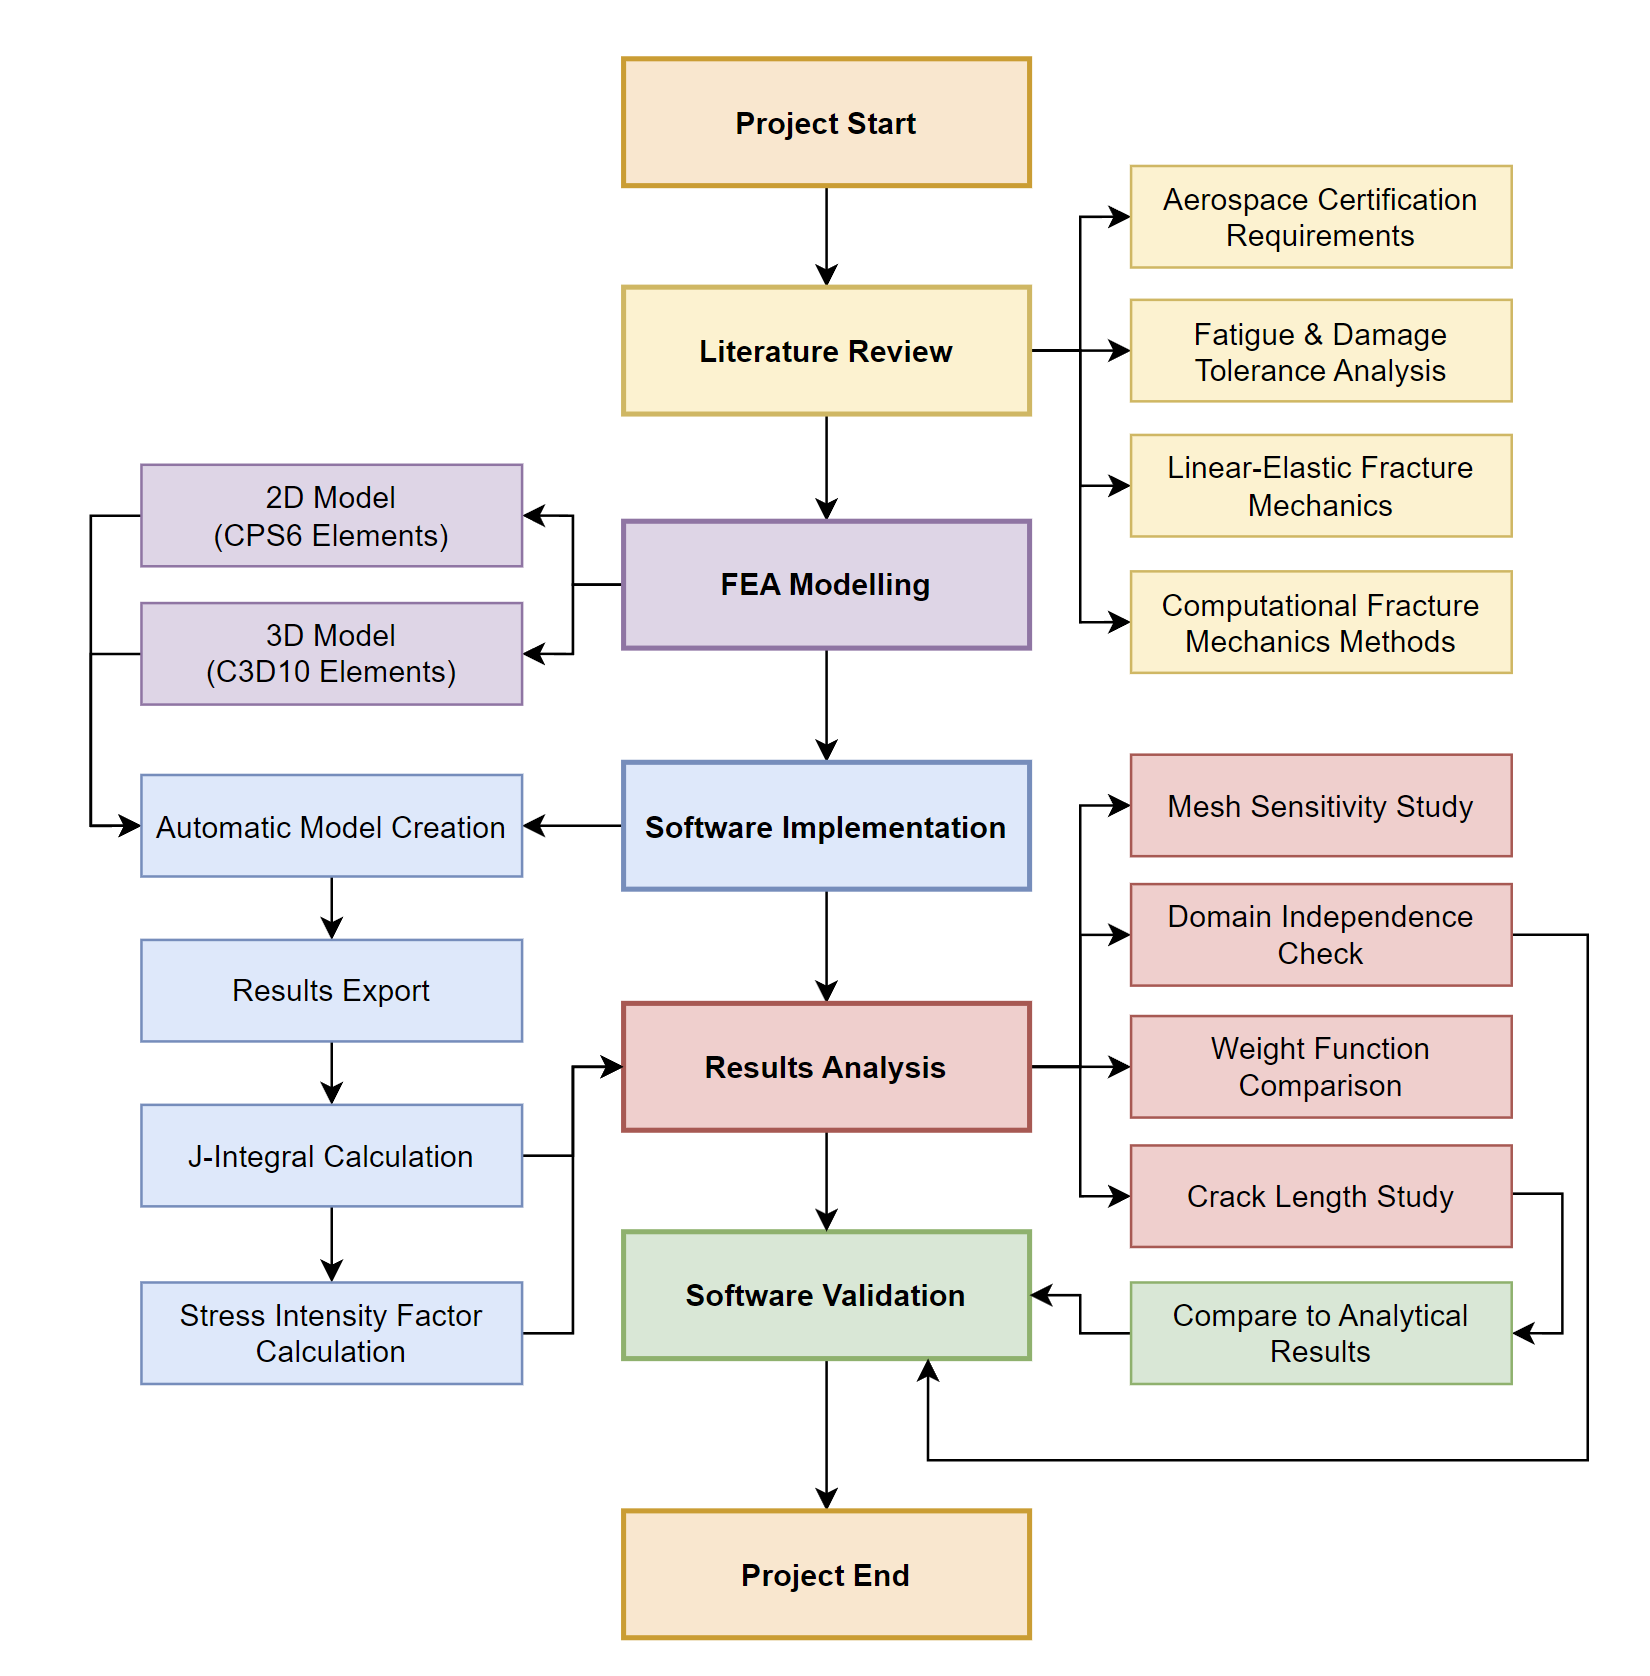
\includegraphics[width=\textwidth]{methodology_diagram.png}
	\caption{Methodology diagram for the project, with sections of the project split by colour, and relationships shown by arrows.}
	\label{fig:methodology_diagram}
\end{figure}

\newpage
\section{Thesis Structure}

Following this introduction, the thesis is separated into four further sections, along with an appendix.

\begin{itemize}
	
	\item Literature Review (§\ref{sec:lit_review}) -- This section details a review of the available literature relevant to the project. Additional context is given on the certification requirements and methods for damage tolerance within the civil aerospace sector. This is followed by a review of the field of linear-elastic fracture mechanics, and a discussion of the most important and relevant relationships. Finally, the application of computational numerical methods to fracture mechanics analysis is discussed.
	
	\item Implementation (§\ref{sec:implementation}) -- This section first details the selection of the most suitable methods and tools for the development of the software, based on the findings of the literature review. The implementation details of the software are then discussed, including the architecture, the creation of the finite element models, the export of the results, and finally the calculation of the stress intensity factor via the J-integral.
	
	\item Results (§\ref{sec:results}) -- This section discusses the validation of the results obtained from the software, using a case study of a through-thickness edge-crack in a finite plate -- in both 2D and in 3D. The rationale behind the selection of suitable parameters for the case study is provided, including the mesh density, weight functions, and integration domains. Finally, the J-integral and stress intensity factor results obtained from the software are compared to analytically-obtained results, in order to verify that the selected method has been implemented correctly, and the results produced via the software are accurate.
	
	\item Conclusion (§\ref{sec:conclusion}) -- This section summarises the project, and discusses how the project was able to meet its original aims and objectives. Some limitations of the selected method and implementation are discussed, and information is provided on the further work necessary to continue the development of the software if it were to be fully realised as a useful analysis tool in the civil aerospace industry.
	
	\item Appendix (§\ref{sec:appendix}) -- This section provides the source code for the software. A link to the GitHub repository for the project is also provided.
	
\end{itemize}